%%%%%%%%%%%%%%%%%%%%%%%%%%%%%%% beamer %%%%%%%%%%%%%%%%%%%%%%%%%%%%%%%%%%%%%%%%%%%%%%%%%
% To run - pdflatex filename.tex
%      acroread filename.pdf
%%%%%%%%%%%%%%%%%%%%%%%%%%%%%%%%%%%%%%%%%%%%%%%%%%%%%%%%%%%%%%%%%%%%%%%%%%%%%%%%%%%%%%%%

\documentclass[compress,oilve]{beamer}
\mode<presentation>

\usetheme[]{CambridgeUS}
% other themes: AnnArbor, Antibes, Bergen, Berkeley, Berlin, Boadilla, boxes, CambridgeUS, Copenhagen, Darmstadt, default, Dresden, Frankfurt, Goettingen,
% Hannover, Ilmenau, JuanLesPins, Luebeck, Madrid, Maloe, Marburg, Montpellier, PaloAlto, Pittsburg, Rochester, Singapore, Szeged, classic

\usecolortheme{beaver}
% color themes: albatross, beaver, beetle, crane, default, dolphin,  fly, lily, orchid, rose, seagull, seahorse, sidebartab, whale, wolverine

\usefonttheme{professionalfonts}
% font themes: default, professionalfonts, serif, structurebold, structureitalicserif, structuresmallcapsserif


\hypersetup{pdfpagemode=FullScreen} % makes your presentation go automatically to full screen

% define your own colors:
\definecolor{Red}{rgb}{1,0,0}
\definecolor{Blue}{rgb}{0,0,1}
\definecolor{Green}{rgb}{0,1,0}
\definecolor{magenta}{rgb}{1,0,.6}
\definecolor{lightblue}{rgb}{0,.5,1}
\definecolor{lightpurple}{rgb}{0.8, 0.6, 0.9}
\definecolor{gold}{rgb}{.6,.5,0}
\definecolor{orange}{rgb}{1,0.4,0}
\definecolor{hotpink}{rgb}{1,0,0.5}
\definecolor{newcolor2}{rgb}{.5,.3,.5}
\definecolor{newcolor}{rgb}{0,.3,1}
\definecolor{newcolor3}{rgb}{1,0,.35}
\definecolor{darkgreen1}{rgb}{0, .35, 0}
\definecolor{darkgreen}{rgb}{0, .6, 0}
\definecolor{darkred}{rgb}{.75,0,0}
\definecolor{skyblue}{HTML}{75bbfd}

\definecolor{olive}{cmyk}{0.64,0,0.95,0.4}
\definecolor{purpleish}{cmyk}{0.75,0.75,0,0}

% can also choose different themes for the "inside" and "outside"

% \usepackage{beamerinnertheme_______}
% inner themes include circles, default, inmargin, rectangles, rounded

% \usepackage{beamerouterthemesmoothbars}
% outer themes include default, infolines, miniframes, shadow, sidebar, smoothbars, smoothtree, split, tree


\useoutertheme[subsection=true, height=40pt]{smoothbars}

% to have the same footer on all slides
%\setbeamertemplate{footline}[text line]{STUFF HERE!}
\setbeamertemplate{footline}[text line]{} % makes the footer EMPTY
% include packages
%

%show the page numbers in footnote
%\addtobeamertemplate{navigation symbols}{}{%
%	\usebeamerfont{footline}%
%	\usebeamercolor[fg]{footline}%
%	\hspace{1em}%
%	\insertframenumber/\inserttotalframenumber
%}

\setbeamercolor{footline}{fg=purpleish}
\setbeamerfont{footline}{series=\bfseries}

%add color to curent subsection
\setbeamertemplate{section in head/foot}{\hfill\tikz\node[rectangle, fill=darkred, rounded corners=1pt,inner sep=1pt,] {\textcolor{white}{\insertsectionhead}};}
\setbeamertemplate{section in head/foot shaded}{\textcolor{darkred}{\hfill\insertsectionhead}}

% Remove bullet of subsections
\setbeamertemplate{headline}
{%
	\begin{beamercolorbox}{section in head/foot}
		\insertsectionnavigationhorizontal{\textwidth}{}{}
	\end{beamercolorbox}%
}


% modify headlline, specially headline size
\setbeamertemplate{headline}{%
	\leavevmode%
	\hbox{%
		\begin{beamercolorbox}[wd=\paperwidth,ht=3.5ex,dp=1.125ex]{palette quaternary}%
			\insertsectionnavigationhorizontal{\paperwidth}{}{\hskip0pt plus1filll}
		\end{beamercolorbox}%
	}
}

\setbeamertemplate{footline}{%
	\leavevmode%
	\hbox{\begin{beamercolorbox}[wd=.5\paperwidth,ht=2.5ex,dp=1.125ex,leftskip=.3cm plus1fill,rightskip=.3cm]{author in head/foot}%
			\usebeamerfont{author in head/foot}\insertshortauthor ~ \insertshortinstitute
		\end{beamercolorbox}%
		\begin{beamercolorbox}[wd=.5\paperwidth,ht=2.5ex,dp=1.125ex,leftskip=.3cm,rightskip=.3cm plus1fil]{title in head/foot}%
			\usebeamerfont{title in head/foot}\insertshorttitle\hfill\insertframenumber\,/\,\inserttotalframenumber
	\end{beamercolorbox}}%
	\vskip0pt%
}


%\setbeamertemplate{navigation symbols}{}

\title{Metrics for classification and regression}
\author{ML Instruction Team, Fall 2022}
\institute[]{CE Department \newline  Sharif University of Technology \newline \newline}
\date[\today]{}
%\titlegraphic{\includegraphics[scale=.35]{example-image}}



%Write \usepackage{etex} just after the \documentclass line (it should be the first loaded package).
\usepackage{etex}
\usepackage{subcaption}
\usepackage{multicol}
\usepackage{amsmath}
\usepackage{epsfig}
\usepackage{graphicx}
\usepackage[all,knot]{xy}
\xyoption{arc}
\usepackage{url}
\usepackage{multimedia}
\usepackage{hyperref}
\hypersetup{colorlinks,linkcolor=blue,citecolor=redorange,urlcolor=darkred}
\usepackage{multirow}
\usepackage[font={scriptsize}]{caption}
\usepackage{pgf}
\usepackage{fontspec}
\usepackage[clean]{svg}

%\setsansfont[Scale=MatchLowercase, BoldFont = * Bold, ItalicFont = * Italic]{Caladea}

%\usepackage{enumitem,xcolor}
%\newcommand{\labelitemi}{$\blacksquare$}
%\newcommand{\labelitemii}{$\diamond$}
%\newcommand{\labelitemiii}{$\square$}
%\newcommand{\labelitemiv}{$\ast$}
%\setbeamercolor*{item}{fg=red}


\usefonttheme{professionalfonts} 
\setbeamertemplate{itemize item}{\color{skyblue}$\blacksquare$}
\setbeamertemplate{itemize subitem}{\color{hotpink}$\blacktriangleright$}
\setbeamertemplate{itemize subsubitem}{\color{orange}$\bullet$}


\usepackage{anyfontsize}
\usepackage{t1enc}
\usepackage{tikz}
\usetikzlibrary{calc,trees,positioning,arrows,chains,shapes.geometric,decorations.pathreplacing,decorations.pathmorphing,shapes,matrix,shapes.symbols}



\newtheorem{proposition}[theorem]{Proposition}
\newtheorem{remark}[theorem]{Remark}
\newtheorem{assumption}[theorem]{Assumption}

\usepackage{fontspec,unicode-math}
\setmainfont{Consolas}[
    Scale=0.9,
    Path=./Fonts/,
    Extension = .ttf,
]
\setmonofont{Monaco}[
    Scale=0.9,
    Path=./Fonts/,
    Extension = .ttf,
]
\definecolor{strings}{rgb}{.624,.251,.259}
\definecolor{keywords}{rgb}{.224,.451,.686}
\definecolor{comment}{rgb}{.322,.451,.322}

\setsansfont[Scale=1]{Times New Roman}

%\usepackage{smartdiagram}
%\usesmartdiagramlibrary{additions}
%%%%%%%%%%%%%%%%%%%%%%%%%%%%%%%%%%%%%%%%%%%%%%%%%%%%%%%%%%%%%%%%%%%%%%%%%%%%%%%%%%%%%%%%%%%%
%%%%%%%%%%%%%%%%%%%%%%%%%%%%%% Title Page Info %%%%%%%%%%%%%%%%%%%%%%%%%%%%%%%%%%%%%%%%%%%
%%%%%%%%%%%%%%%%%%%%%%%%%%%%%%%%%%%%%%%%%%%%%%%%%%%%%%%%%%%%%%%%%%%%%%%%%%%%%%%%%%%%%%%%%%


%%%%%%%%%%%%%%%%%%%%%%%%%%%%%%%%%%%%%%%%%%%%%%%%%%%%%%%%%%%%%%%%%%%%%%%%%%%%%%%%%%%%%%%%%%
%%%%%%%%%%%%%%%%%%%%%%%%%%%%%% Begin Your Document %%%%%%%%%%%%%%%%%%%%%%%%%%%%%%%%%%%%%%%
%%%%%%%%%%%%%%%%%%%%%%%%%%%%%%%%%%%%%%%%%%%%%%%%%%%%%%%%%%%%%%%%%%%%%%%%%%%%%%%%%%%%%%%%%%
\begin{document}
	
%%%%%%%%%%%%%%%%%%%%%%%%%%%%%%%%%%%%%%%%%%%%%%%%%%%%%%%%%%%%%%%%%%%%%%%%%%%%%%%%%%%%%%%%%%
	\fontsize{9}{9}
\begin{frame}[noframenumbering, plain]
	\titlepage
\end{frame}

%%%%%%%%%%%%%%%%%%%%%%%%%%%%%%%%%%%%%%%%%%%%%%%%%%%%%%%%%%%%%%%%%%%%%%%%%%%%%%%%%%%%%%%%%%
\section{Recap}
%%%%%%%%%%%%%%%%%%%%%%%%%%%%%%%%%%%%%%%%%%%%%%%%%%%%%%%%%%%%%%%%%%%%%%%%######
\frame{\frametitle{MNIST Dataset}
\begin{center}
    \begin{figure}
        \centering
        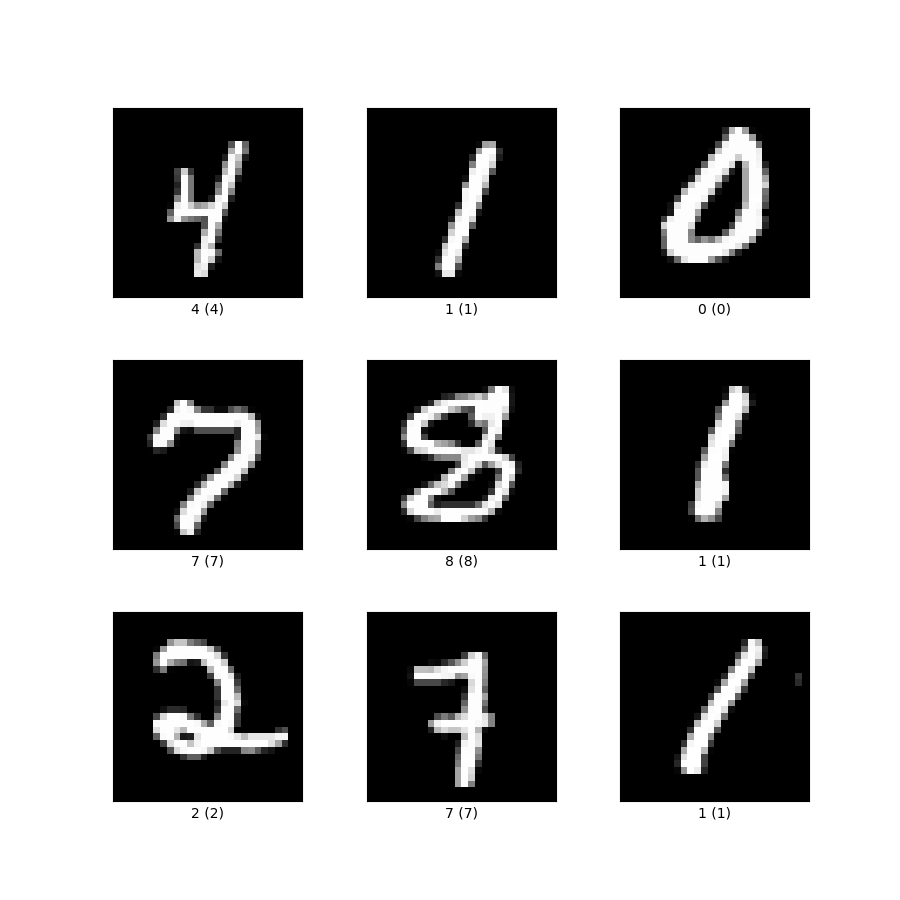
\includegraphics[width=0.5\columnwidth]{Figs/mnistDataset.png}
        \caption{MNIST dataset}
    \end{figure}
\end{center}


% \begin{itemize}
% 	\item One
% 	\begin{itemize}
% 		\item One
% 		\item Two
% 		\item Three
% 	\end{itemize}

% 	\item 
% 	For two-dimensional tensors, we have a corresponding sum with indices $(a, b)$ for $f$ and $(i-a, j-b)$ for $g$, respectively:
% 	$$
% 	(f * g)(i, j)=\sum_a \sum_b f(a, b) g(i-a, j-b)
% 	$$
	
% 	\item 
	
% 	It is given by,
% 	$$
% 	\left.w_{t+1}=w_t-\left(\alpha_t / \sqrt{\left(v_t\right.}\right)+e\right) *\left(\delta L / \delta w_t\right)
% 	$$
% 	where,
% 	$$
% 	v_t=\beta * v_t+(1-\beta) *\left(\delta L / \delta w_t\right)^2
% 	$$
% \end{itemize}	
	
}
\section{Classification Metrics}

\frame{\frametitle{Never5 Classifier}
	\begin{itemize}
		\item Suppose a very dumb classifier that just classifies every single image in the “not-5” class.
		\item It will achieve a accuracy around \textbf{90\%}.
		\item Accuracy is not always a good measurment.
	\end{itemize}	
}

\frame{\frametitle{Confusion Matrix}
	\begin{center}
    \begin{figure}
        \centering
        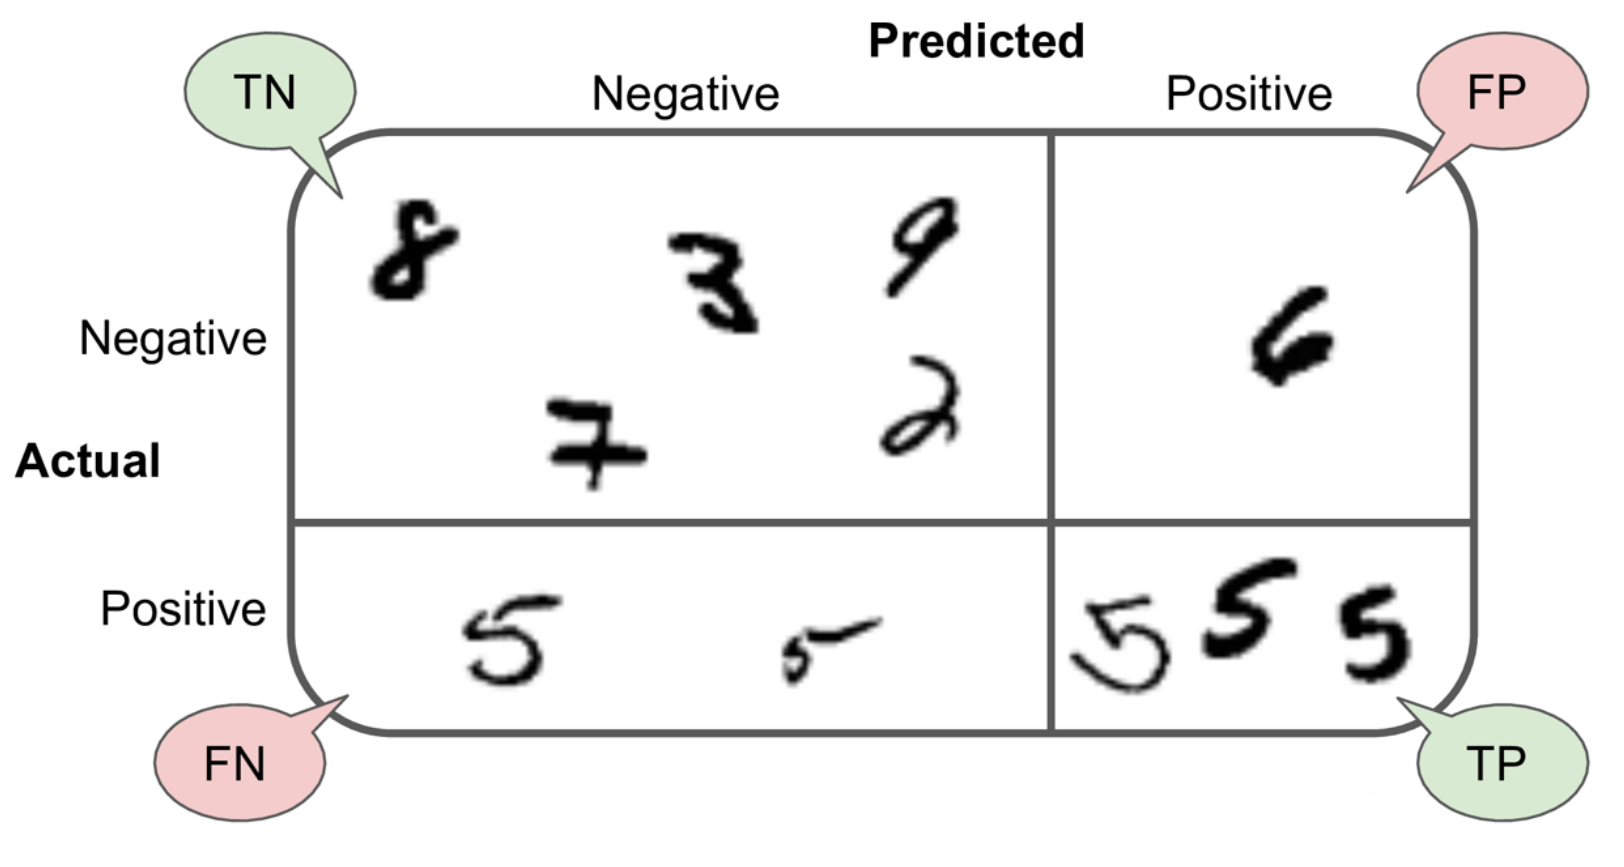
\includegraphics[width=0.5\columnwidth]{Figs/confMatrix.jpg}
        \caption{Confusion Matrix For a Classifier}
    \end{figure}
    \begin{center}
    \begin{equation}
    \begin{split}
    ERR = \frac{FP + FN}{FP + FN + TP + TN} = 1 - ACC
    \end{split}
    \end{equation}
    \end{center}
    \begin{center}
    \begin{equation}
    \begin{split}
    ACC = \frac{TP + TN}{FP + FN + TP + TN} = 1 - ERR
    \end{split}
    \end{equation}
    \end{center}
\end{center}	
}

%%%%%%%%%%%%%%%%%%%%%%%%%%%%%%%%%%%%%%%%%%%%%%%%%%%%%%%%%%%%%%%%%%%%%%%%%%%%%%%%%%%%%%%%%%%%%%%

\frame{\frametitle{False Positive Rate and False Negative Rate}
	\begin{center}
    \begin{equation}
    \begin{split}
    TPR = \frac{TP}{P} = \frac{TP}{TP + FN} = 1 - FNR
    \end{split}
    \end{equation}
    \end{center}
    \begin{center}
    \begin{equation}
    \begin{split}
    FPR = \frac{FP}{N} = \frac{FP}{FP + TN} = 1 - TNR
    \end{split}
    \end{equation}
    \end{center}
    \begin{center}
    \begin{equation}
    \begin{split}
    FNR = \frac{FP}{N} = \frac{FN}{FN + TP} = 1 - TPR
    \end{split}
    \end{equation}
    \end{center}
    \begin{center}
    \begin{equation}
    \begin{split}
    TNR = \frac{TN}{N} = \frac{TN}{TN + FP} = 1 - FPR
    \end{split}
    \end{equation}
    \end{center}
}

\frame{\frametitle{Precision, Recall, F_{1} Score}
	\begin{center}
    \begin{figure}
        \centering
        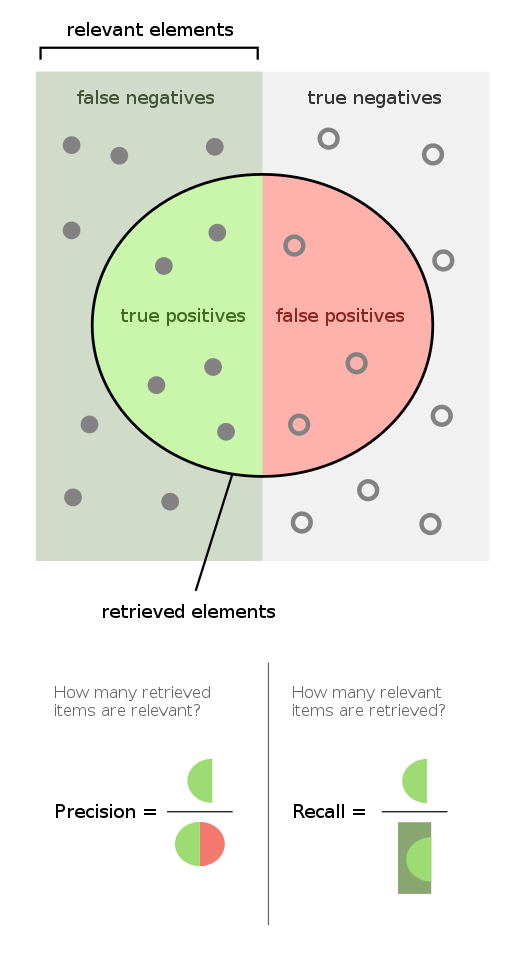
\includegraphics[width=0.3\columnwidth]{Figs/Precisionrecall.png}
        \caption{\href{https://en.wikipedia.org/wiki/Precision_and_recall}{source}}
    \end{figure}
    \end{center}
}

\frame{\frametitle{Precision, Recall, F_{1} Score}
	\begin{itemize}
		\begin{center}
        \begin{equation}
        \begin{split}
        PRE = \frac{TP}{TP + FP}
        \end{split}
        \end{equation}
        \end{center}
        \begin{center}
        \begin{equation}
        \begin{split}
        REC = TPR = \frac{TP}{FN + TP}
        \end{split}
        \end{equation}
        \end{center}
        \begin{center}
        \begin{equation}
        \begin{split}
        F_{1} = 2.\frac{PRE.REC}{PRE + REC}
        \end{split}
        \end{equation}
        \end{center}
	\end{itemize}
		
}


\frame{\frametitle{Decision Threshold}
	\begin{center}
    \begin{figure}
        \centering
        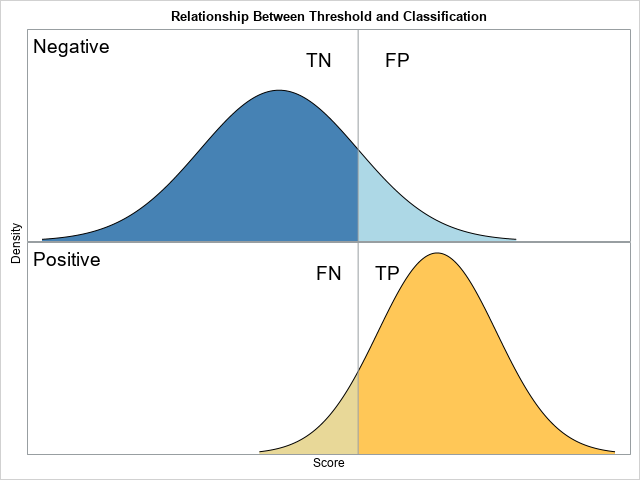
\includegraphics[width=0.6\columnwidth]{Figs/classifyTNFP2.png}
        \caption{\href{https://blogs.sas.com/content/iml/2020/02/24/binary-classification-viz.html}{source}}
    \end{figure}
    \end{center}
}


\frame{\frametitle{Precision/Recall Trade-off}
	\begin{center}
    \begin{figure}
        \centering
        \includegraphics[width=0.9\columnwidth]{Figs/decionfuncion.png}
        \caption{the higher the threshold, the lower the recall, but (in general) the higher the precision}
    \end{figure}
    \end{center}
}

\frame{\frametitle{Precision/Recall Trade-off}
	\begin{center}
    \begin{figure}
        \centering
        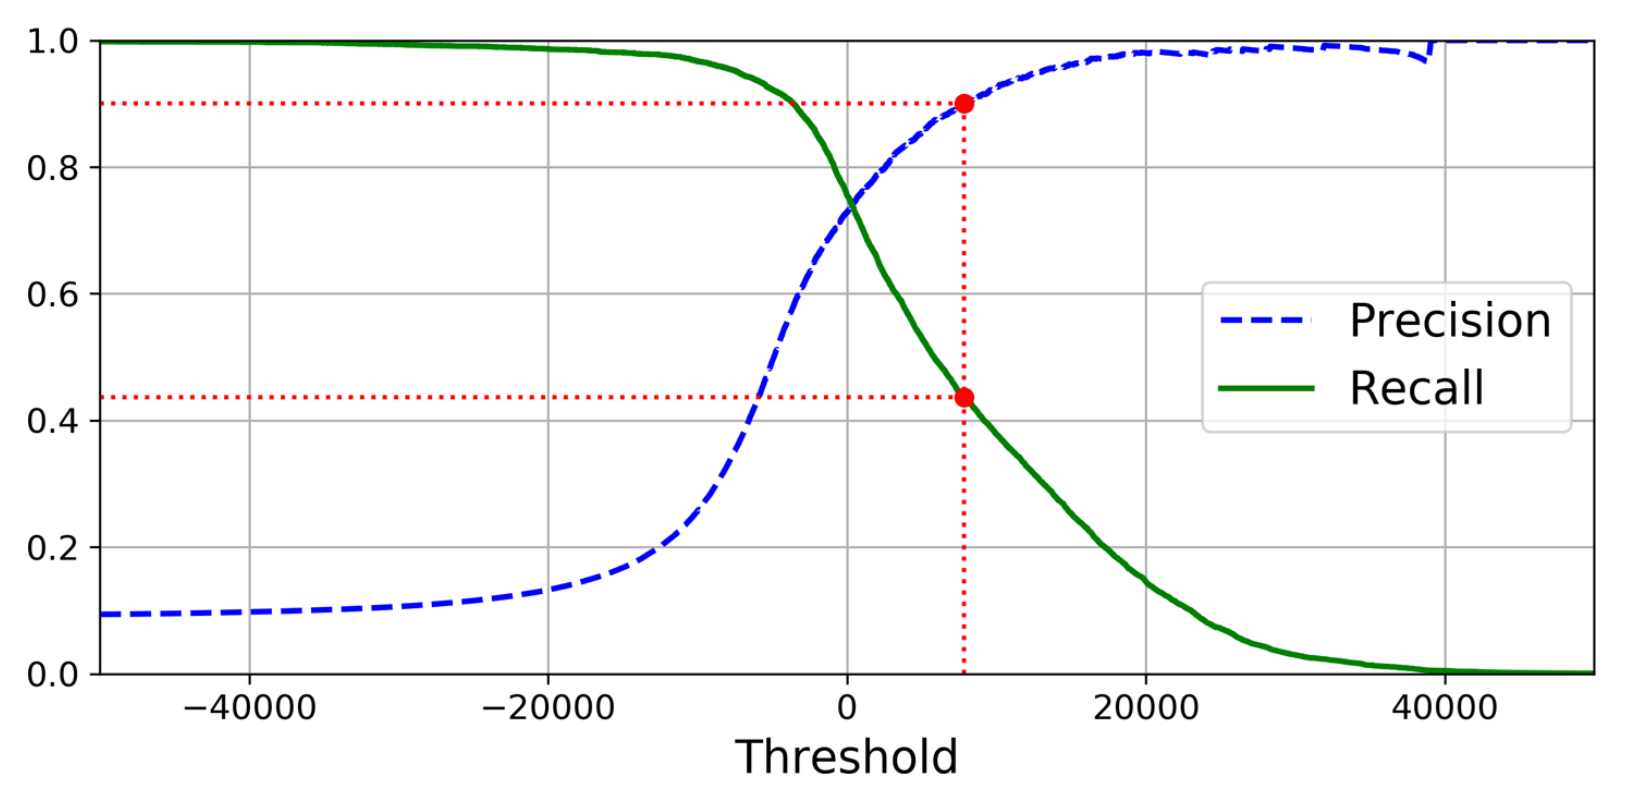
\includegraphics[width=0.9\columnwidth]{Figs/decisionFunction2.png}
        \caption{Precision and recall versus the decision threshold}
    \end{figure}
    \end{center}
}

\frame{\frametitle{Sensitivity and Specificity}
    \begin{itemize}
	\begin{center}
    \begin{equation}
    \begin{split}
    SEN = TPR = \frac{TP}{P} = \frac{TP}{TP + FN}
    \end{split}
    \end{equation}
    \end{center}
    
    \begin{center}
    \begin{equation}
    \begin{split}
    SPC = TNR = \frac{TN}{N} = \frac{TN}{TN + FP}
    \end{split}
    \end{equation}
    \end{center}
    \newline
    \item Sensitivity (SEN) measures the recovery rate of the Positives and complimentary.
    \item Specificity (SPC) measures the recovery rate of negatives.
    \end{itemize}
}


\frame{\frametitle{ROC Curve}
	\begin{itemize}
		\item plots the \emp{true positive rate} against \emp{false positive rate}.
		\item used with binary classifiers.
	\end{itemize}	
}


\frame{\frametitle{ROC Curve}
	\begin{center}
    \begin{figure}
        \centering
        \includegraphics[width=0.75\columnwidth]{Figs/ROC.png}
        \caption{ROC Curve}
    \end{figure}
    \end{center}
}

\frame{\frametitle{Area Under The Curve (AUC)}
	\begin{itemize}
		\item another way to compare classifiers.
		\item perfect classifier has a ROC AUC equal to 1.
	\end{itemize}	
}

\frame{\frametitle{Area Under The Curve (AUC)}
	\begin{center}
    \begin{figure}
        \centering
        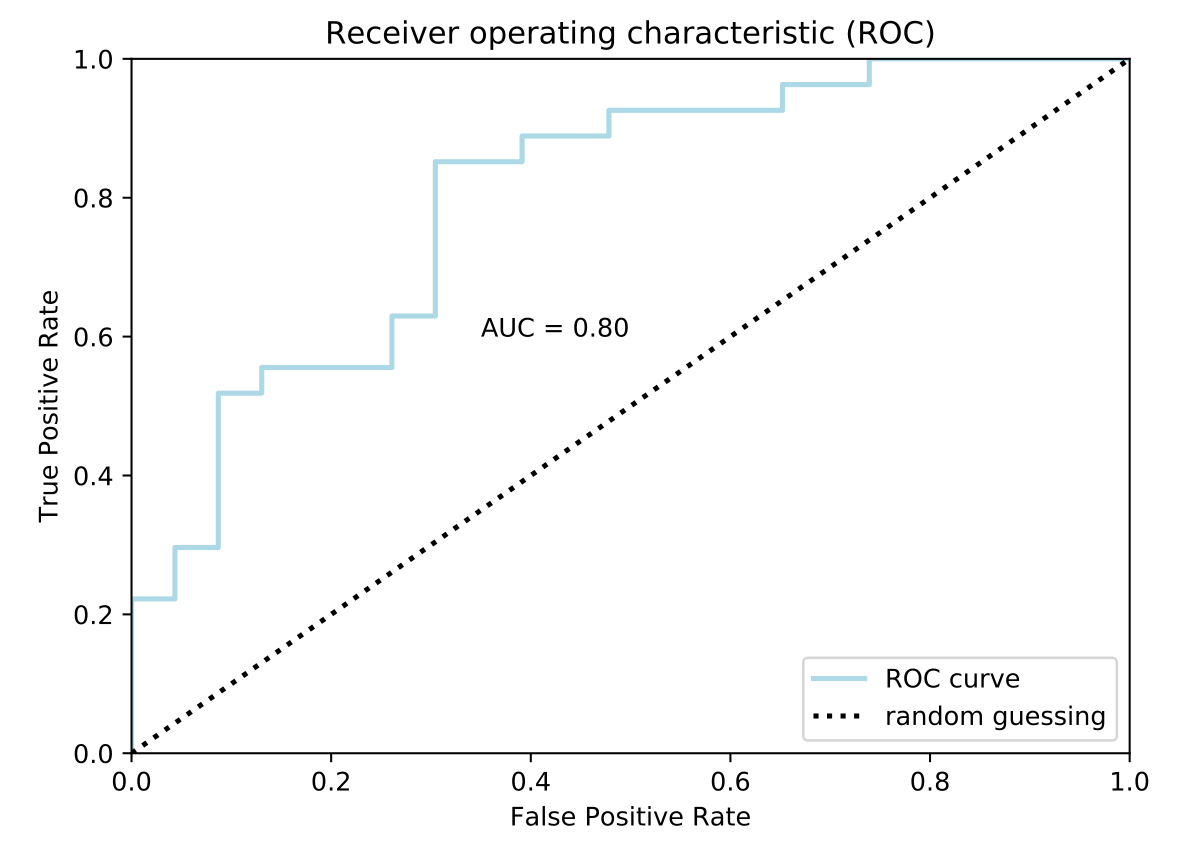
\includegraphics[width=0.75\columnwidth]{Figs/AUC.png}
        \caption{ROC AUC}
    \end{figure}
    \end{center}
}

\section{Regression Metrics}

\frame{\frametitle{Root Mean Squared Error (RMSE)}
	\begin{itemize}
		\item a metric for regressors.
		\item perfect regressor has a RMSE equal to 0.
		\begin{center}
        \begin{equation}
        \begin{split}
        RMSE = \sqrt{(\frac{1}{n})\sum_{i=1}^{n}(y_{i} - \hat{y_{i}})^{2}}
        \end{split}
        \end{equation}
        \end{center}
	\end{itemize}	
}

\frametitle{Final Notes}
\centering
\vspace{50 pt}
\textbf{Thank You!}
\vspace{50pt}

\textbf{Any Question?}
%%%%%%%%%%%%%%%%%%%%%%%%%%%%%%%%%%%%%%%%%%
\end{document}